\chapter{Evaluation} \label{cha:evaluation}

This chapter evaluates the outcome of the migration process.
% The outcome of the migration process is evaluated in the fifth chapter. The potential benefits and drawbacks of the serverless platform outlined in chapter 2 are used to reflect on the final artifact. The chapter includes approximations on measurable attributes such as hosting costs and performance as well as discussion on the more subjective attributes like maintainability and testability. The overall ease of development -- or developer experience -- is also addressed since it is one of the commonly reported pain points of serverless computing

% Finally in chapter \ref{cha:evaluation} the migration outcome is evaluated against the pre-migration application in terms of quality and ease of development.
Evaluation the outcome of migration process. Estimate the effects on performance and hosting costs. Weigh in on maintainability, testability, developer experience etc.

\section{Developer perspective}

development ease, operations, maintainability

From a development point of view the process of rewriting server application code into FaaS function handlers was found relatively simple. The same runtime environment (NodeJS v10) was used in both versions of the application and the deployment artifacts for both were built from the same codebase. The server application's code also benefited from being modularized so that the server-specific request handling implementation was separated from image processing logic, for example. These factors together enabled a high degree of code reuse when implementing FaaS functions. The source code of the image labeling function is presented in listing \ref{lst:labelerhandler} to exemplify how a comparatively small amount of boilerplate code is required to instantiate a new function: in this function the labeling logic is imported from a \textit{label} module which is also used as-is by the server application.

\begin{lstlisting}[language=JavaScript,caption=Image labeler function handler,captionpos=b,label=lst:labelerhandler,showstringspaces=false,belowskip=2em,frame=tb,aboveskip=2em]
  import { Storage } from '@google-cloud/storage'
  import { getBucketFileLabels } from '../label'

  const gcs = new Storage()

  export async function labeler(data) {
    const labels = await getBucketFileLabels(data)

    return gcs
      .bucket(data.bucket)
      .file(data.name)
      .setMetadata({ metadata: { Labels: labels } })
  }
\end{lstlisting}

Developing and testing the functions locally was found more challenging, depending on function type. In case of the authorizer function local development was simple since the function exposes a synchronous HTTP API, behaving the same as a conventional server application. In that case a local development server could be used to mimic a deployed function without any mocking or test harnesses required. Developing the other functions locally was more difficult due to their event-driven invocation style, which meant that the triggering cloud events would have to be replicated locally. Without any tooling in place to mock cloud events, for these functions it was found easier to deploy them to the cloud and develop against the actual deployed functions. While the deployment process was relatively fast, this did incur a degree of overhead in the development cycle.



qualitative vs quantitative

% check example at https://onlinelibrary.wiley.com/doi/epdf/10.1002/spe.2608
How did the migration help in future extendability and maintenance of Image Manager?
- development perspective
  - less bundling/coupling
- operational perspective
  - ease of deployment
  - monitoring
- financial perspective
- performance perspective
  - cold start averted by 1) optionally using function warmer, 2) only having one synchronous bottleneck, otherwise event-driven
- others?

Old implementation's shortcomings of availability, scalability, cost-efficiency and isolation -- we're these addressed?

Maintainability. The modular architecture of micro-services  allows  reducing  the  complexity  of  mono-lithic  systems.  Breaking  a  system  into  independent  and    self-deployable    services    enables    developer    teams  to  make  changes  and  test  their  service  independent  of  other  developers,  which  simplifies  distributed  development.  Moreover,  the  small  size  of  each  microservice  contributes  to  increasing  code understandability,  and  thus  to  improving  the  maintainability of the code.
Scalability. Scaling microservices is easier than scaling  monoliths.  Scaling  monolithic  systems  requires  huge  investment  in  terms  of  hardware  and  often  finetuning  of  the  code.  If  there  is  a  bottleneck  in  some  component,  a  more  powerful  piece  of  hardware can be used, or multiple instances of the same monolithic  application  can  be  executed  across  several services and managed by a load balancer.In   contrast,   microservices   are   not   automatically  scalable,  even  if  they  are  commonly  deployed  in  elastic  and  stateless  architectures.  However,  in  a  microservicesbased  system,  each  microservice  can  be deployed on a different server, with different levels of  performance,  and  can  be  written  in  the  most  appropriate  development  language.  If  there  is  a  bottleneck  in  one  microservice  in  such  a  case,  the  specific microservice can be containerized and executed across multiple hosts in parallel, without the need to deploy the whole system to a more powerful machine.

% got more or less cloud-ready? \parencite{pozdniakova17cloudready}

\section{Performance perspective}

\section{Economic perspective}

\begin{figure}[h]
  \centering
  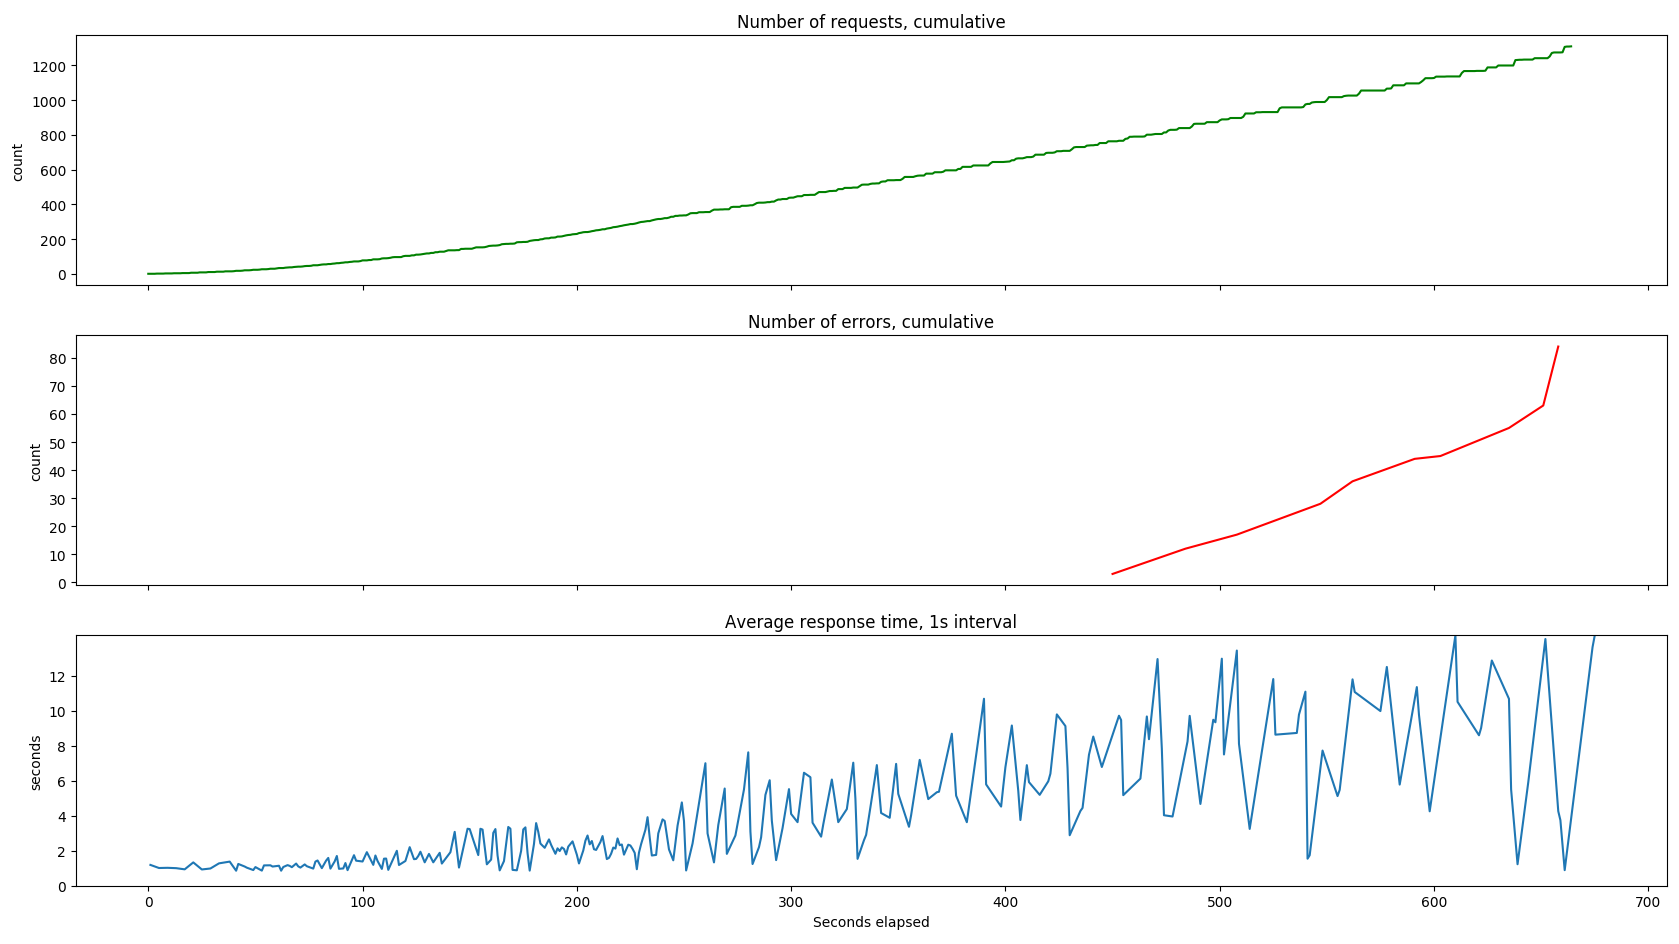
\includegraphics[width=0.9\textwidth]{serverful-load-test.png}
  \caption{Serverful Image Manager load test results}
  \label{fig:serverfulLoadTest}
\end{figure}

\begin{figure}
  \centering
  \begin{subfigure}[b]{0.9\textwidth}
      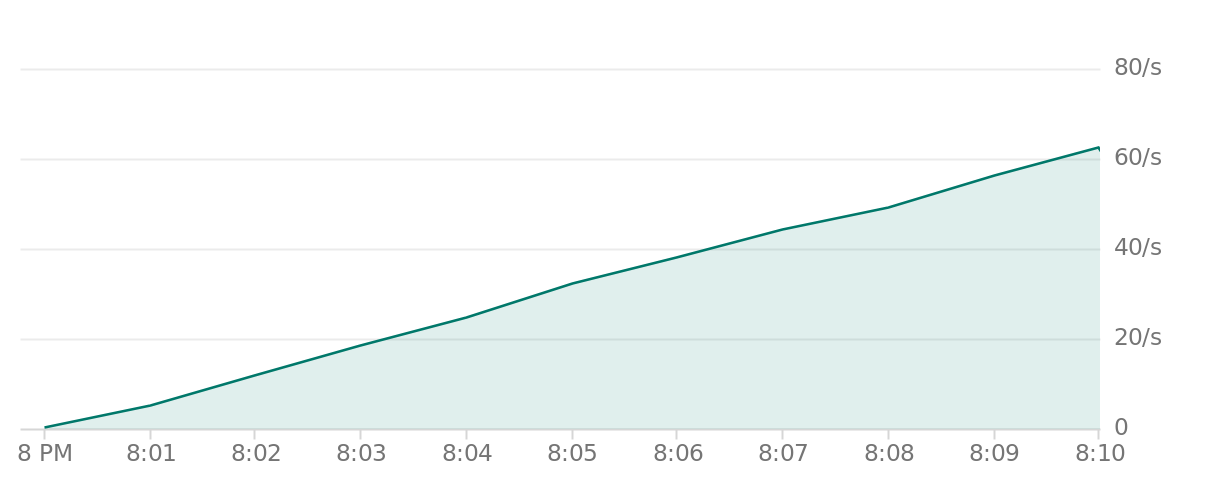
\includegraphics[width=\textwidth]{cloud-functions-invocations-per-second.png}
      \caption{Invocations per second, sum of all functions}
      \label{fig:tiger}
  \end{subfigure}

  \begin{subfigure}[b]{0.9\textwidth}
      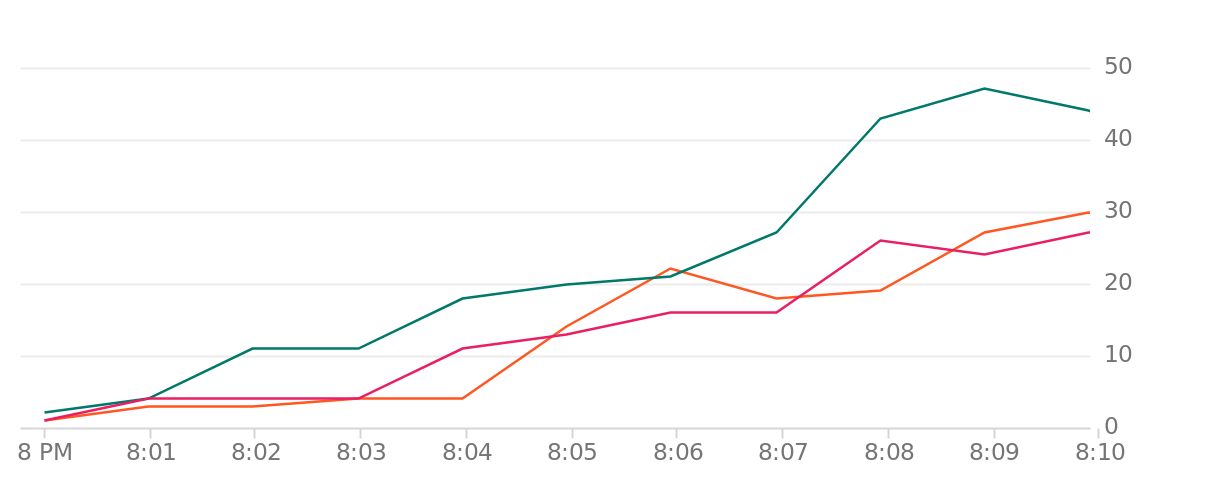
\includegraphics[width=\textwidth]{cloud-function-active-instances.png}
      \caption{Active instances per function}
      \label{fig:gull}
  \end{subfigure}

  \begin{subfigure}[b]{0.9\textwidth}
      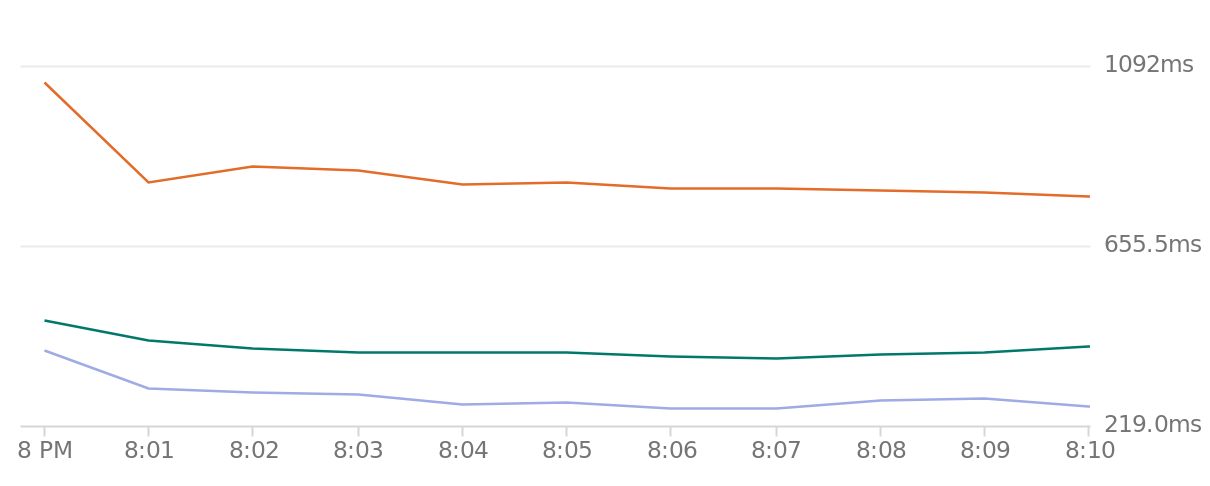
\includegraphics[width=\textwidth]{cloud-function-execution-times-mean.png}
      \caption{Mean execution times per function}
      \label{fig:mouse}
  \end{subfigure}
  \caption{Serverless Image Manager load test results}\label{fig:serverlessLoadTest}
\end{figure}

